%%%%%%%%%%%%%%%%%%%%%%%%%%%%%%%%%%%%%%%%%%%%%%%%%%%%%%%%
%%%
%%%  LaTeX template for Junior Journal article
%%%  Please don't change next few lines
%%%
%%%%%%%%%%%%%%%%%%%%%%%%%%%%%%%%%%%%%%%%%%%%%%%%%%%%%%%%

\documentclass{juniorjournal}
%\setcounter{page}{}
%\journaltitle{}
%\volume{}
%\pubyear{}
%\licensee{}
%\authorlist{}
%\doi{}
%\articlenumber{}
%\articletype{}

%%%%%%%%%%%%%%%%%%%%%%%%%%%%%%%%%%%%%%%%%%%%%%%%%%%%%%%%
%%% 
%%%  List custom packages below, if needed. 
%%%  Note that amsfonts,amstext,amssymb,amsmath,amsthm,amscd
%%%  bm,paralist,color,graphicx,array and subfigure packages
%%%  are all part of juniorjournal.cls
%%%
%%%%%%%%%%%%%%%%%%%%%%%%%%%%%%%%%%%%%%%%%%%%%%%%%%%%%%%%

\usepackage{listings}
\usepackage{hyperref}

\definecolor{javared}{rgb}{0.6,0,0} % for strings
\definecolor{javagreen}{rgb}{0.25,0.5,0.35} % comments
\definecolor{javapurple}{rgb}{0.5,0,0.35} % keywords
\definecolor{javadocblue}{rgb}{0.25,0.35,0.75} % javadoc

\lstset{language=Java,
basicstyle=\ttfamily,
keywordstyle=\color{javapurple}\bfseries,
stringstyle=\color{javared},
commentstyle=\color{javagreen},
morecomment=[s][\color{javadocblue}]{/**}{*/},
numbers=left,
numberstyle=\tiny\color{black},
stepnumber=2,
numbersep=10pt,
tabsize=4,
showspaces=false,
showstringspaces=false}

%%%%%%%%%%%%%%%%%%%%%%%%%%%%%%%%%%%%%%%%%%%%%%%%%%%%%%%%
%%%
%%%  Journal article basic info.
%%%  List all authors first and then their affiliations. 
%%%  Link author and affiliations with numbers in optional arguments.
%%%  For corresponding author use the form given below.
%%%  
%%%  For example:
%%%  \author[1]{Name1 Surname1}
%%%  \author[2, \corresp]{Name2 Surname2}\correspemail{email@edu.com}
%%%  \affil[1]{Institute1, Country1}
%%%  \affil[2]{Institute2, Country2}
%%%  
%%%%%%%%%%%%%%%%%%%%%%%%%%%%%%%%%%%%%%%%%%%%%%%%%%%%%%%%

\articletitle{LinkJVM 2.0 - Java on the KIPR Link} % To break lines in long titles use \\

%\author[ ,\corresp]{}\correspemail{}
\author[1, \corresp]{Markus Klein}\correspemail{m@mklein.co.at}
\author[1]{Christoph Hackenberger}
\affil[1]{Vienna Institute of Technology}
%%%%%%%%%%%%%%%%%%%%%%%%%%%%%%%%%%%%%%%%%%%%%%%%%%%%%%%%
%%%
%%%  Main document.
%%%
%%%  To span floating objects (wide images, tables, etc.)
%%%  over twocolumn layout, use figure* 
%%%  or table* environments.
%%%
%%%  Examples:
%%%  \begin{figure*}	 \begin{table*}		
%%%   ...				  ...				
%%%  \end{figure*}		 \end{table*}		
%%%
%%%%%%%%%%%%%%%%%%%%%%%%%%%%%%%%%%%%%%%%%%%%%%%%%%%%%%%%

\begin{document}
\maketitle

\articleabstract{}
\keywords{Java, JVM, Botball, Library, Framework, Wrapper, KIPR Link, Libkovan, Robotic, JNI, SWIG, JamVM, GNU Classpath, Open Source}

\section{Introduction}
The purpose of Botball is to motivate students for building and programming autonomous robots.
Most new students to Botball do not have any experience with programming.
Therefore the way of developing the robot software has to be very beginner friendly and easy to use, 
but at the same time very powerful.

So what is the best language for Botball?
The authors do not think there is a best choice.
Every language has its own advantages and disadvantages.
C for example is a very powerful fast and processor-near language so it is quite good for a robot 
controller doing a lot of basic things such as controlling servos and motors, reading sensor values 
and so on. 
But for students who have not yet learned anything about programming or how a computer works, 
it would be very hard to learn and understand C code. 
If you want to develop a complex C program, you have to know how pointer arithmetic and memory 
access works.

Another well-known possibility is Java. 
Java is much easier to learn and also pretty powerful and reliable.
Of course it is not as fast as compiled languages such as C or C++, 
but in the most cases it will make no real difference.
Java is better for beginners, 
compared to C it does not require special knowledge about how a computer works.
Java is a higher level language.
It provides automatic garbage collection to handle memory management 
and offers an excellent set of basic data structures such as lists, queues and maps.
In C everything has to be built from scratch.
The object-oriented paradigm is also very helpful to structure the program 
to improve the maintainability.

In most schools in Austria students get started with programming using Java and not C or C++.
Therefore the authors would consider themselves as a good Java programmer, 
but they never wrote a bigger project using C.

Further alternatives are event-based frameworks using a scripting language 
such as node or in general scripting languages, but these can be implemented very easily, 
because the JVM(Java Virtual Machine) supports a huge amount of additional languages 
including javascript, scala and clojure.
%\lstinputlisting[language=Java]{listings/Debugger.java}

\section{State of the Art}
LinkJVM 1.0 was published at the Global Conference on Educational Robotics 2013 (GCER 2013).
While the Java environment JamVM and GNU Classpath work pretty well the robot library is not that good.
At that time LinkJVM 1.0 wraps over libkovan's C bindings which makes the libary structure pretty poor, because LinkJVM first calls the native C function and then the native C function manages the C++ objects.
Is approach is in easier to implement, but it also comes with some downsides.
The most important of them is that there no possibility to write a thread save library using this approach, because libkovan itself is not thread-save.
Moreover LinkJVM 1.0 offers only a very small API with much less features that libkovan does and LinkJVM's vision system contains also just one camera class.
Therefor the authors decided to write a new library from scratch which will fix all this issues. 

\section{Design Approach}
\label{sec:design-approach}
The framework of the LinkJVM consists of one high and one low level part.
The low level part of the LinkJVM wraps the existing C++ library of libkovan, 
the high level now wraps the low level part and represents the API for the user.
So the user only uses the high level part of the LinkJVM and should not come in 
contact with any low level things.

\begin{figure}[htbp]
\centering
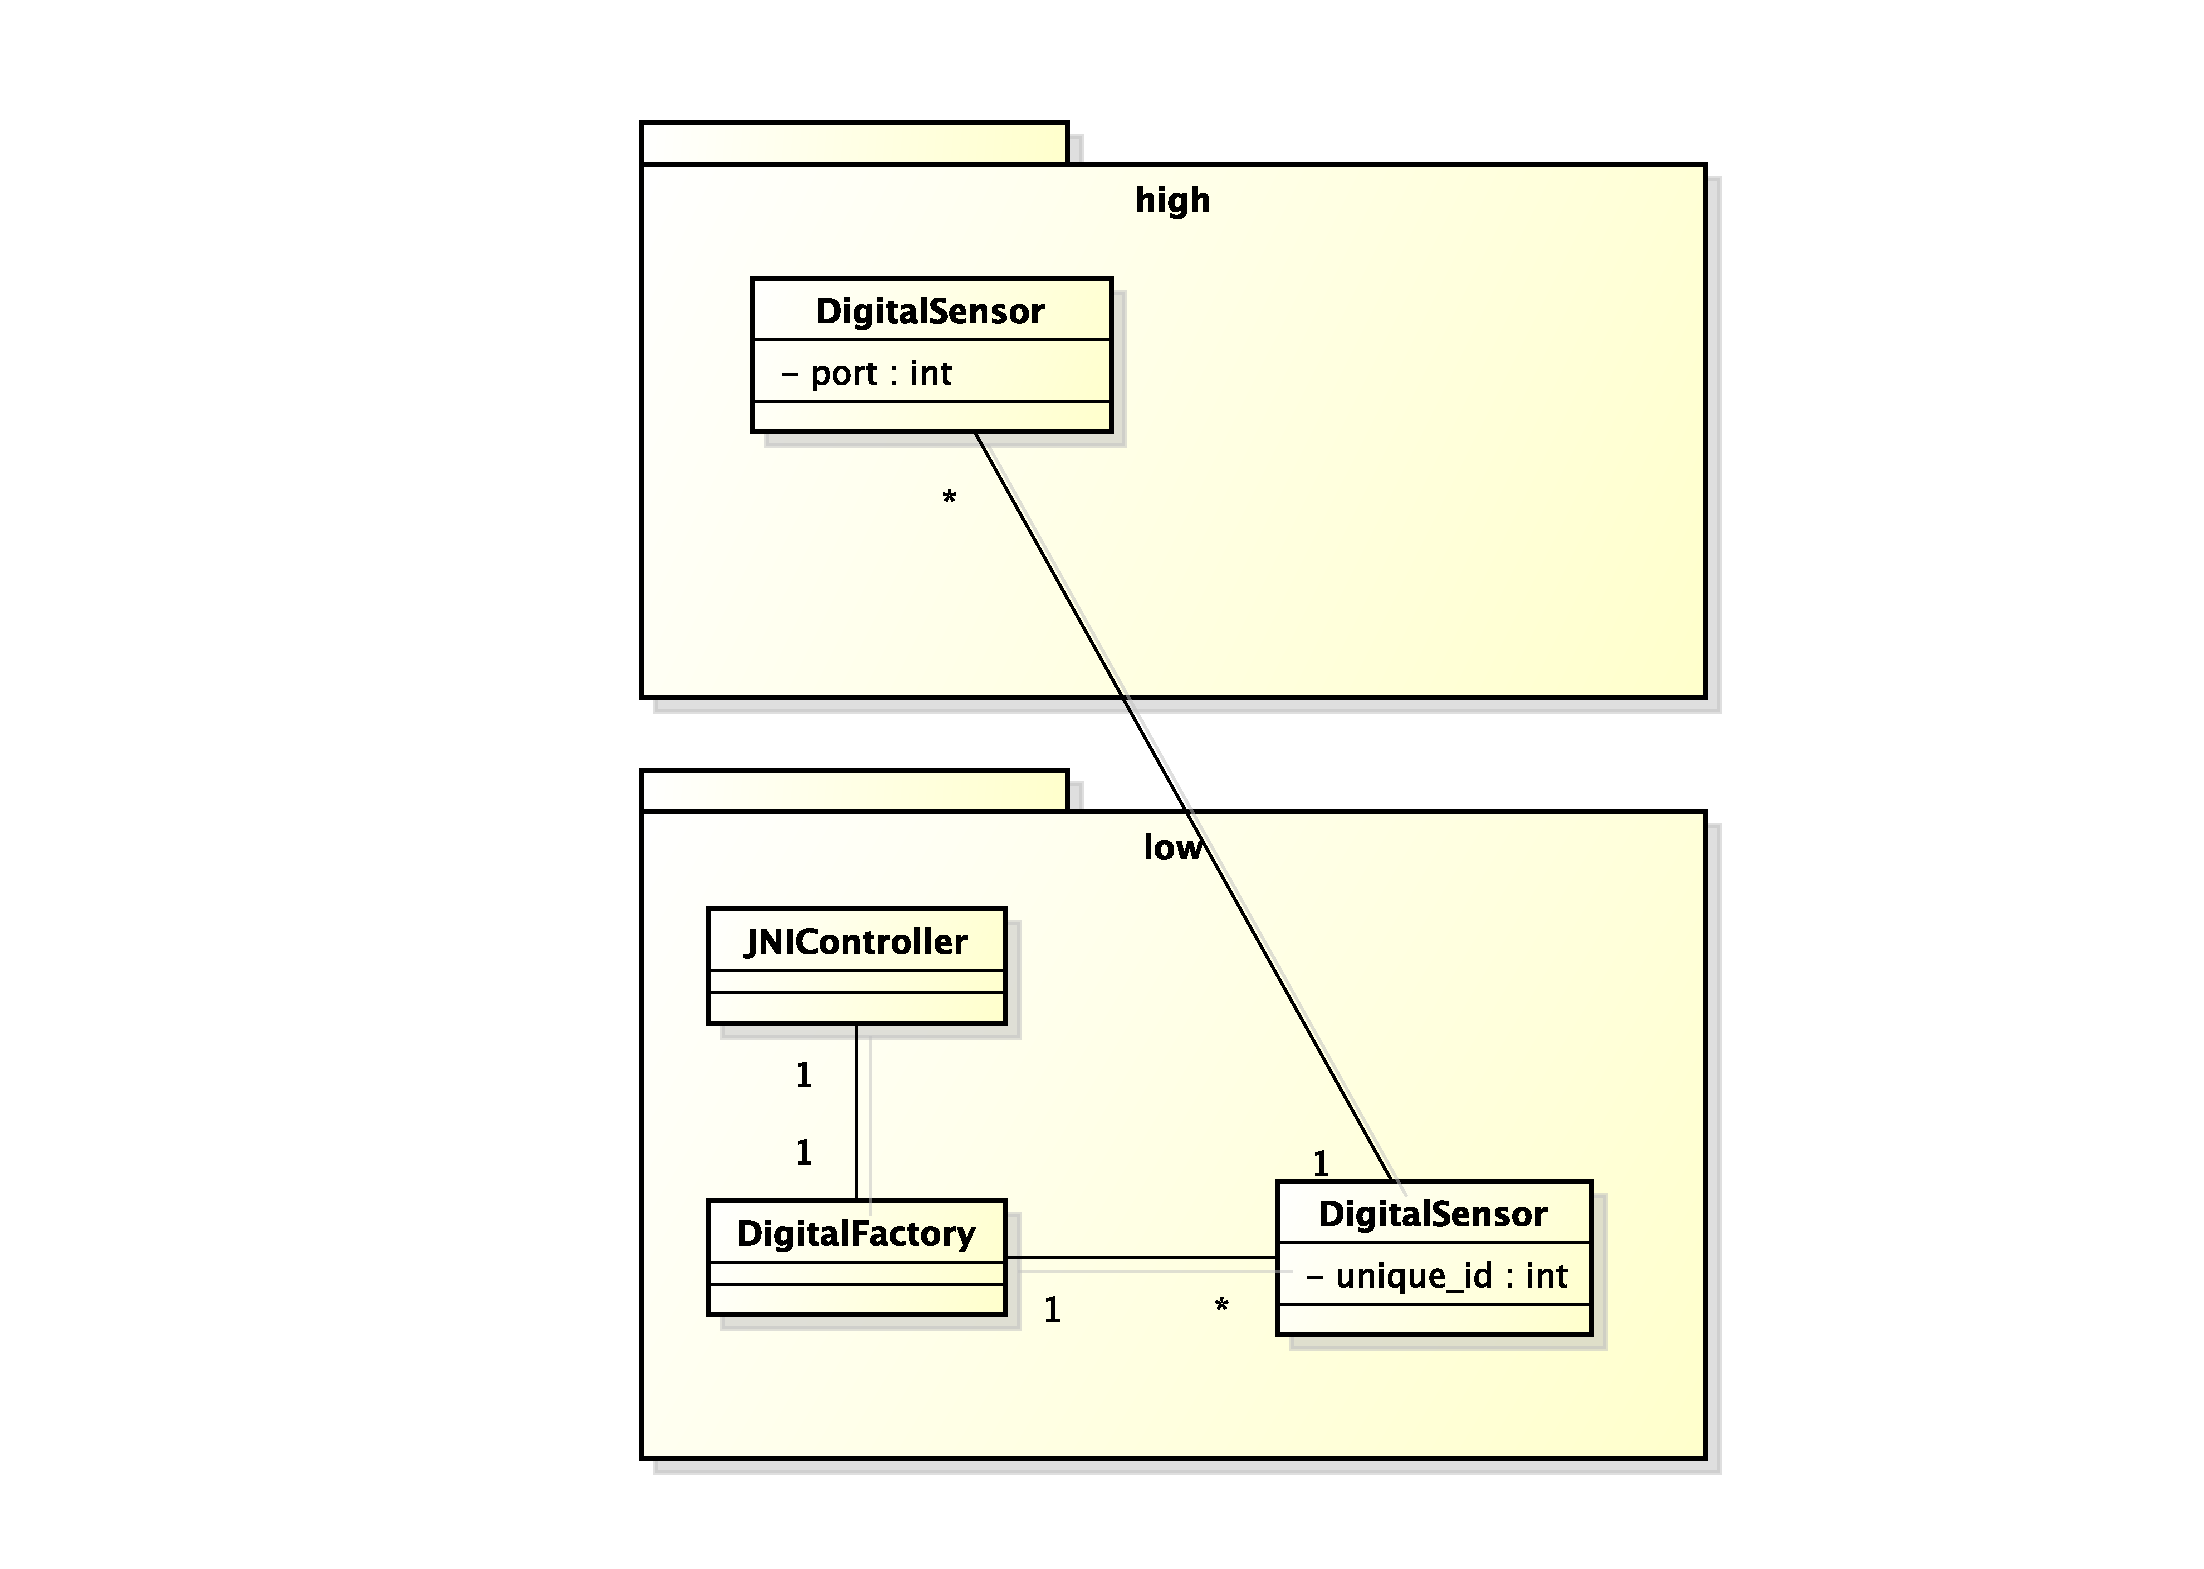
\includegraphics[width=0.5\textwidth]{images/Class-Diagram.pdf}
\caption{Class-Diagram}
\label{fig:Class-Diagram}
\end{figure}

For example the user has a digital sensor like a lever on his robot and now 
wants to use this sensor in his program. He will now create a new high level 
DigitalSensor object, which uses a low level DigitalSensor object in the 
backround (see Figure \ref{fig:Class-Diagram}) that again uses the C++ implementation of a DigitalSensor.

\begin{figure}[htbp]
\centering
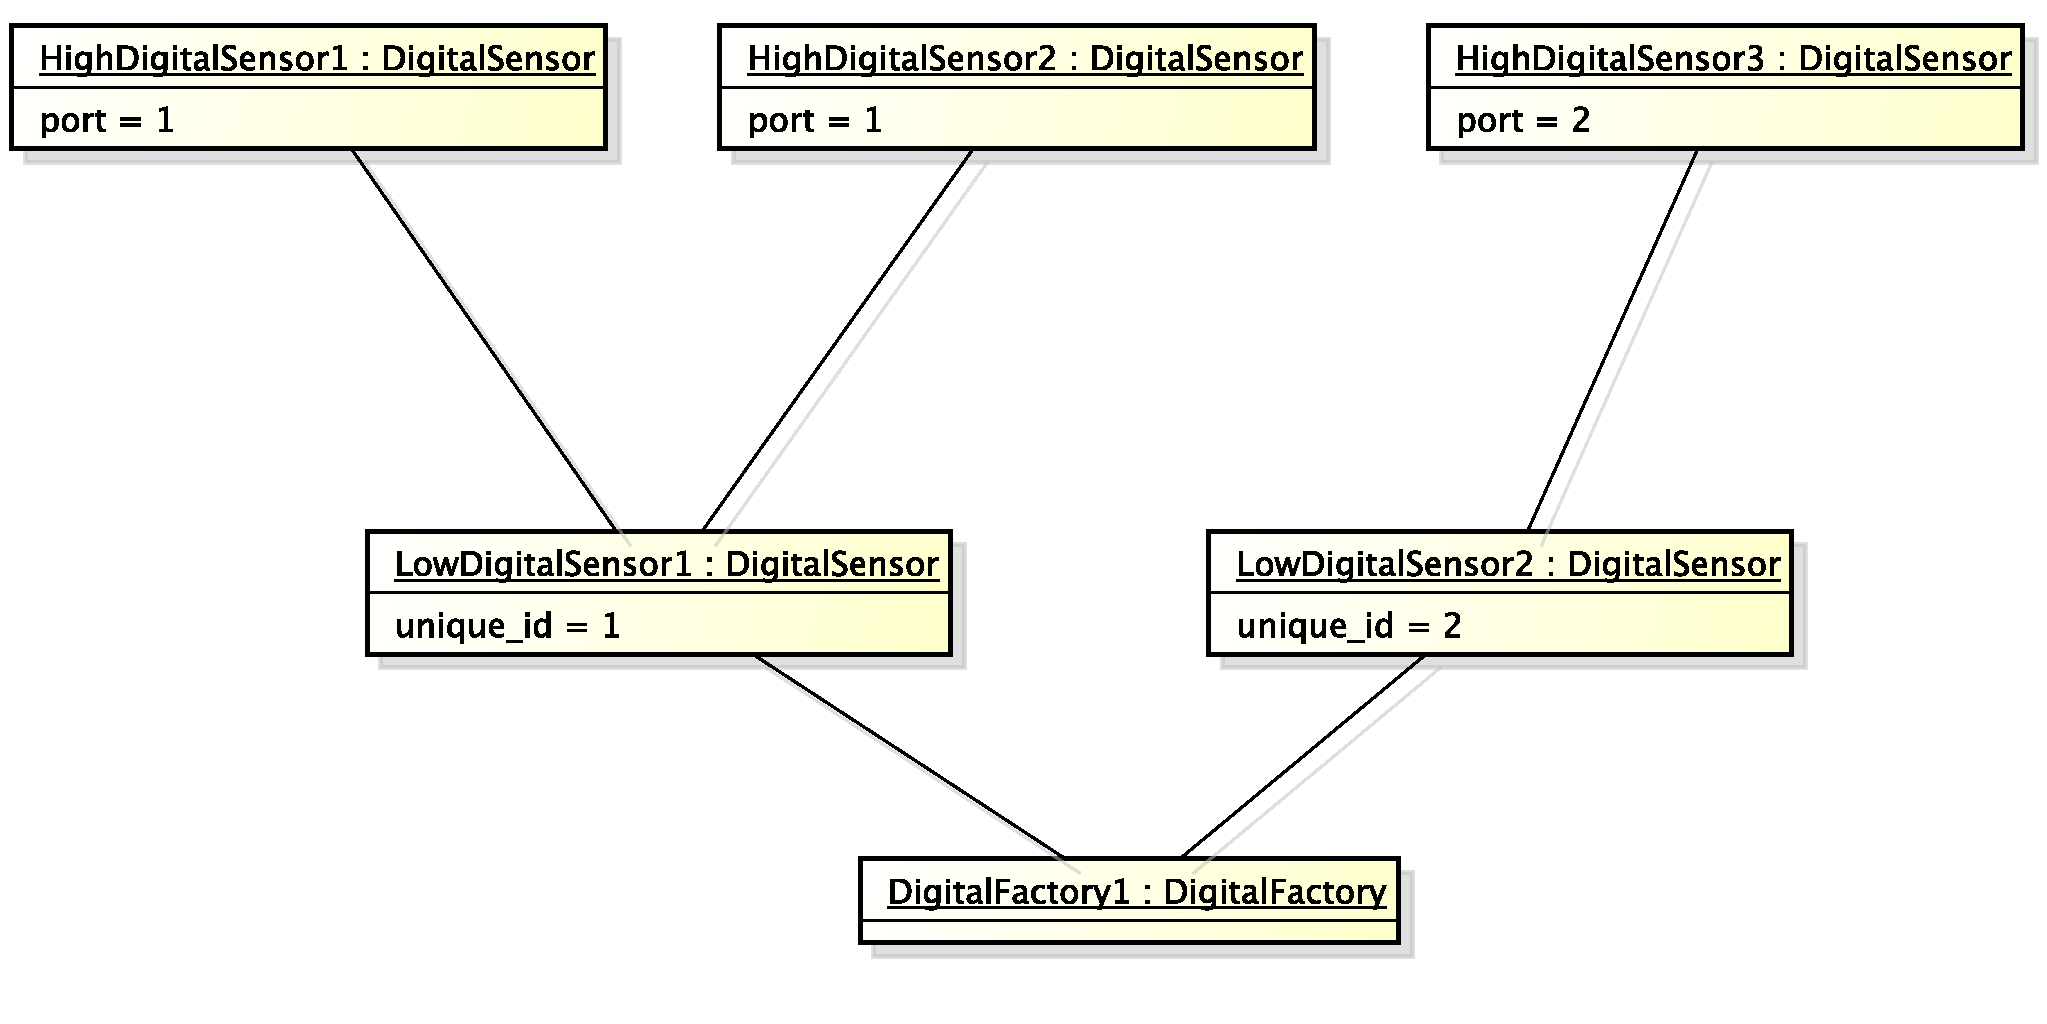
\includegraphics[width=0.5\textwidth]{images/Object-Diagram.pdf}
\caption{Object-Diagram}
\label{fig:Object-Diagram}
\end{figure}

The user can create as much high level objects of the same sensor, motor, 
servo,... , which will all uses the same low level object with the specified 
unique identifier, which is for example the port of a sensor. If the user 
creates a new high level object with a unique identifier that is unequal to 
an existing low level object the appropriate factory would 
create a new low level object with the specified unique identifier. (see figure \ref{fig:Object-Diagram})

Both the low and the high level parts are described in detail in the following subsections:

\subsection{Low Level}
The low level part of the framework contains the java side libkovan wrapper. 
Every object of a low level class is also a native c++ object.
This classes must be instanciated using the corresponding multiton factory, which means that every low object has a unique identifier as described in section \nameref{sec:design-approach}.
The low level part also provieds the JNIController class which holds a singleton of every factory as well as one static singleton object of itself.

\subsection{High Level}
The high level part contains, as already mentioned before, the API for the user. 
Internally every time the user creates a new high level object, the high object requests a new low object.
See figure \ref{fig:Class-Diagram} and figure \ref{fig:Object-Diagram} for more details.
\section{Java Environment}
LinkJVM includes a Java Runtime Environment(JRE) which consists of a lightweight Java Virtual Machine(JVM) and GNU Classpath an open source implementation of the java core classes.
Moreover it also offeres a Java compiler(javac) for compiling java source code as well as jar for packaging compiled class files.
\subsection{JamVM}

\section{Developing Tools}
Because the code the user writes with the LinkJVM library uses the programming 
language Java, it is not possible to use the KISS IDE from KIPR because it only 
supports C or C++ code.

The authors decided to leave the choice of how to write the code at the user. It 
is possible to write the code with an IDE like Eclipse or Netbeans or just write 
it in a simple text editor and compile the source code over the console.

\begin{figure}[htbp]
\centering
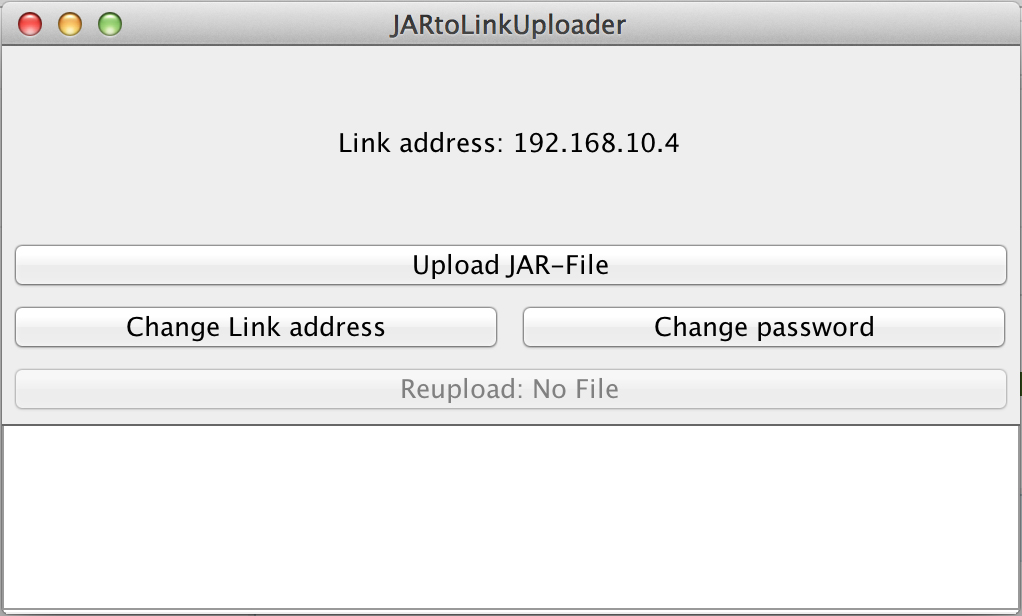
\includegraphics[width=0.5\textwidth]{images/linkjvm_uploader.jpg}
\caption{LinkJVM-Uploader}
\label{fig:linkjvm_uploader}
\end{figure}

At the beginning it was only possible to upload/run you program via scp/ssh to/on the KIPR Link.
Running a program over ssh is not tournament-conformal, so the only thing that could be done 
was to write a C wrapper, which executes your java program.

So the next logical thing the authors have to think about is how to get the compiled 
program on the KIPR Link and make it run able there in a for the user easy way?
They first thinked about a plugin for the Eclipse IDE but this would extremely 
limit the user of how to write the code, which like already mentioned the 
authors wanted to leave the choice at the user.
The authors decided to write an independent program, which is called 
LinkJVM-Uploader or JARtoLinkUploader (see Figure \ref{fig:linkjvm_uploader}), 
to upload .jar files to the link. This program also automatically creates C 
wrappers, which executes the .jar files and which are shown in the menu point 
'Programs' on the KIPR Link. All this is done over ssh and scp connections in 
the background.

\begin{thebibliography}{500} % Include .bib (.bbl) references here

\end{thebibliography}

\end{document}
